
\begin{table}
\renewcommand{\arraystretch}{0.7}
 \begin{tabular}{l rm{7em} rm{7em} rm{7em}}
\hline \hline \\

{} & \multicolumn{2}{c}{2008 Presidential} & \multicolumn{2}{c}{2012 Presidential} & \multicolumn{2}{c}{2016 Presidential} \\

\\ \hline \\
107th Congress         &   6.0 &          \includegraphics[width=7em]{mini_hist/MN_2008_107} &   5.0 &          \includegraphics[width=7em]{mini_hist/MN_2012_107} &   3.0 &          \includegraphics[width=7em]{mini_hist/MN_2016_107} \\
111th Congress         &   5.0 &          \includegraphics[width=7em]{mini_hist/MN_2008_111} &   5.0 &          \includegraphics[width=7em]{mini_hist/MN_2012_111} &   3.0 &          \includegraphics[width=7em]{mini_hist/MN_2016_111} \\
114th Congress         &   6.0 &          \includegraphics[width=7em]{mini_hist/MN_2008_114} &   6.0 &          \includegraphics[width=7em]{mini_hist/MN_2012_114} &   3.0 &          \includegraphics[width=7em]{mini_hist/MN_2016_114} \\
\\ \hline \\ 
Areal Distance         &   5.3 &       \includegraphics[width=7em]{mini_hist/MN_2008_dist_a} &   5.2 &       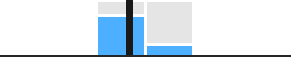
\includegraphics[width=7em]{mini_hist/MN_2012_dist_a} &   3.2 &       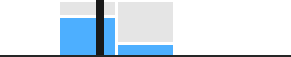
\includegraphics[width=7em]{mini_hist/MN_2016_dist_a} \\
Axis Ratio             &   5.8 &   \includegraphics[width=7em]{mini_hist/MN_2008_axis_ratio} &   5.3 &   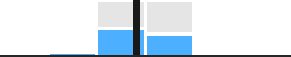
\includegraphics[width=7em]{mini_hist/MN_2012_axis_ratio} &   3.6 &   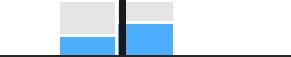
\includegraphics[width=7em]{mini_hist/MN_2016_axis_ratio} \\
Circumscribing Circles &   5.7 &        \includegraphics[width=7em]{mini_hist/MN_2008_reock} &   5.4 &        \includegraphics[width=7em]{mini_hist/MN_2012_reock} &   3.5 &        \includegraphics[width=7em]{mini_hist/MN_2016_reock} \\
Distance to Perimeter  &   5.9 &     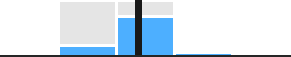
\includegraphics[width=7em]{mini_hist/MN_2008_rohrbach} &   5.5 &     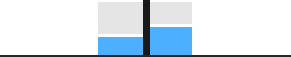
\includegraphics[width=7em]{mini_hist/MN_2012_rohrbach} &   3.8 &     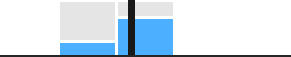
\includegraphics[width=7em]{mini_hist/MN_2016_rohrbach} \\
Dynamic Radius         &   5.6 &   \includegraphics[width=7em]{mini_hist/MN_2008_dyn_radius} &   5.2 &   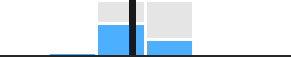
\includegraphics[width=7em]{mini_hist/MN_2012_dyn_radius} &   3.4 &   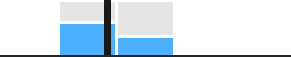
\includegraphics[width=7em]{mini_hist/MN_2016_dyn_radius} \\
Exchange               &   5.6 &     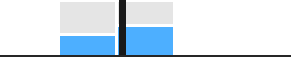
\includegraphics[width=7em]{mini_hist/MN_2008_exchange} &   5.3 &     \includegraphics[width=7em]{mini_hist/MN_2012_exchange} &   3.5 &     \includegraphics[width=7em]{mini_hist/MN_2016_exchange} \\
Harmonic Radius        &   5.4 &  \includegraphics[width=7em]{mini_hist/MN_2008_harm_radius} &   5.0 &  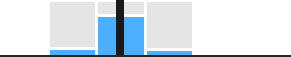
\includegraphics[width=7em]{mini_hist/MN_2012_harm_radius} &   3.2 &  \includegraphics[width=7em]{mini_hist/MN_2016_harm_radius} \\
Hull Area              &   6.1 &       \includegraphics[width=7em]{mini_hist/MN_2008_hull_a} &   5.8 &       \includegraphics[width=7em]{mini_hist/MN_2012_hull_a} &   4.0 &       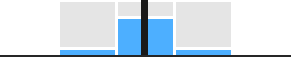
\includegraphics[width=7em]{mini_hist/MN_2016_hull_a} \\
Hull Population        &   5.5 &       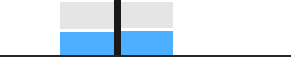
\includegraphics[width=7em]{mini_hist/MN_2008_hull_p} &   5.1 &       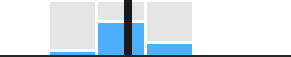
\includegraphics[width=7em]{mini_hist/MN_2012_hull_p} &   3.4 &       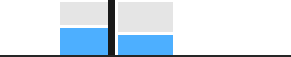
\includegraphics[width=7em]{mini_hist/MN_2016_hull_p} \\
Inertia Area           &   5.5 &    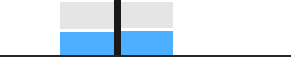
\includegraphics[width=7em]{mini_hist/MN_2008_inertia_a} &   5.2 &    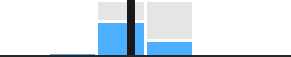
\includegraphics[width=7em]{mini_hist/MN_2012_inertia_a} &   3.4 &    \includegraphics[width=7em]{mini_hist/MN_2016_inertia_a} \\
Inertia Population     &   5.8 &    \includegraphics[width=7em]{mini_hist/MN_2008_inertia_p} &   5.5 &    \includegraphics[width=7em]{mini_hist/MN_2012_inertia_p} &   3.6 &    \includegraphics[width=7em]{mini_hist/MN_2016_inertia_p} \\
Inscribed Circles      &   5.7 &    \includegraphics[width=7em]{mini_hist/MN_2008_ehrenburg} &   5.0 &    \includegraphics[width=7em]{mini_hist/MN_2012_ehrenburg} &   3.4 &    \includegraphics[width=7em]{mini_hist/MN_2016_ehrenburg} \\
Isoperimeter Quotient  &   5.7 &       \includegraphics[width=7em]{mini_hist/MN_2008_polsby} &   5.2 &       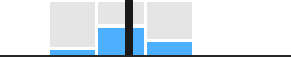
\includegraphics[width=7em]{mini_hist/MN_2012_polsby} &   3.5 &       \includegraphics[width=7em]{mini_hist/MN_2016_polsby} \\
Mean Radius            &   5.6 &  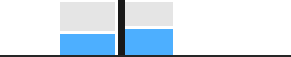
\includegraphics[width=7em]{mini_hist/MN_2008_mean_radius} &   5.2 &  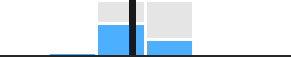
\includegraphics[width=7em]{mini_hist/MN_2012_mean_radius} &   3.4 &  \includegraphics[width=7em]{mini_hist/MN_2016_mean_radius} \\
Path Fraction          &   5.7 &    \includegraphics[width=7em]{mini_hist/MN_2008_path_frac} &   5.1 &    \includegraphics[width=7em]{mini_hist/MN_2012_path_frac} &   3.5 &    \includegraphics[width=7em]{mini_hist/MN_2016_path_frac} \\
Population Distance    &   5.7 &       \includegraphics[width=7em]{mini_hist/MN_2008_dist_p} &   5.4 &       \includegraphics[width=7em]{mini_hist/MN_2012_dist_p} &   3.5 &       \includegraphics[width=7em]{mini_hist/MN_2016_dist_p} \\
Power Diagram          &   5.4 &        \includegraphics[width=7em]{mini_hist/MN_2008_power} &   5.2 &        \includegraphics[width=7em]{mini_hist/MN_2012_power} &   3.2 &        \includegraphics[width=7em]{mini_hist/MN_2016_power} \\
Split-Line             &   6.0 &        \includegraphics[width=7em]{mini_hist/MN_2008_split_ax} &   6.0 &        \includegraphics[width=7em]{mini_hist/MN_2012_split_ax} &   4.0 &        \includegraphics[width=7em]{mini_hist/MN_2016_split_ax} \\
\hline \hline
\end{tabular}
\caption{Votes from presidential elections in Minnesota are aggregated from precinct-level returns, into maps simulated with each algorithm or compactness metric. 
             The seats expected to accrue to Democrats (mean across maps) are displayed numerically as well as by a solid black line.
             The normalized distribution of seats per metric/algorithm is shown in blue and the 10-90\% range of possible seats is highlighted in gray.
             The same re-aggregation is performed for enacted maps used for the 107th, 111th, and 114th Congresses and shown in red.
             Since reapportionment shifts the number of seats per state,
               the entries for the 107th and 111th Congresses are the Democratic share,
               times the 8 assigned after the 2010 Census.
             }\label{tab:MN_seats}
\end{table}
 